
The enclosure will be difficult to construct for multiple reasons.  In order to
minimize the size of the PCB, we decided to forgo traditional mounting holes.
Additionally, we would like to avoid using adhesive to mount the PCB in order
to maintain easy access for debugging purposes.  This means the enclosure will
need tight tolerances around the PCB to prevent horizontal movement.  Vertical
movement can be easily countered by sandwiching the PCB between the bottom and
top half of the enclosure.  Additionally, the sensors mounted on the bottom on
the PCB need to be a precise distance away from the users wrist.  This means
the thickness of the bottom of the enclosure needs to accurately tuned.

To add difficulty to the situation, the enclosure is to be manufactured by a
(rather cheap) desktop FDM 3D printer.  These printers are known for over
extruding plastic which causes the produces part to be slightly larger in the X
and Y dimensions.  As over extruding is preferable to under extruding, it is
common to simply model the part slightly smaller to compensate.

FDM printers also tend to warp parts if the plastic cools too quickly, but that
can be countered by simply putting the printer in a warm room or giving the
printer a cozy blanket (although that is a fire hazard).

However, FDM 3D printing is exceptionally fast.  They make it possible to
iterate and print a 3D model of this size multiple times per day.  This rapid
iteration will allow me to create parts that meet the above requirements.

The need for rapid iteration has led to the creation of many parametric 3D
modeling programs.  The idea is to define variables (like the the thickness of
the bottom of the model) that can easily be changed.  The problem with many of
these modeling programs is that they simply save a series of steps the user has
entered with the GUI so they can later replay this with different values.  This
replay of events is very error prone and usually requires a lot of human
intervention.  This is because the interface makes it difficult to specify
geometry that is valid for a wide parameter range.

For this reason, I've decided to use OpenSCAD.  OpenSCAD defines 3D models in
its scripting language which is executed to produce 3D printable files.  Since
every usage of a parameter is written out explicitly, it is easy to determine
all the valid values for the parameters.

The current state of the model can be seen in figure \ref{fig:enclosure}.  It
is only a simple box with appropriate nubs sticking out to accept a watch band.
The parameters that can currently be adjusted are the wall thickness, PCB size,
and watch band width.  Going forward I will add a parameter for over extrusion
used to adjust the X and Y dimensions so I can perfectly seat the PCB.  I will
also have to finish modeling the rest of the watch geometry.

\begin{figure}
\centering
\makebox[\textwidth]{
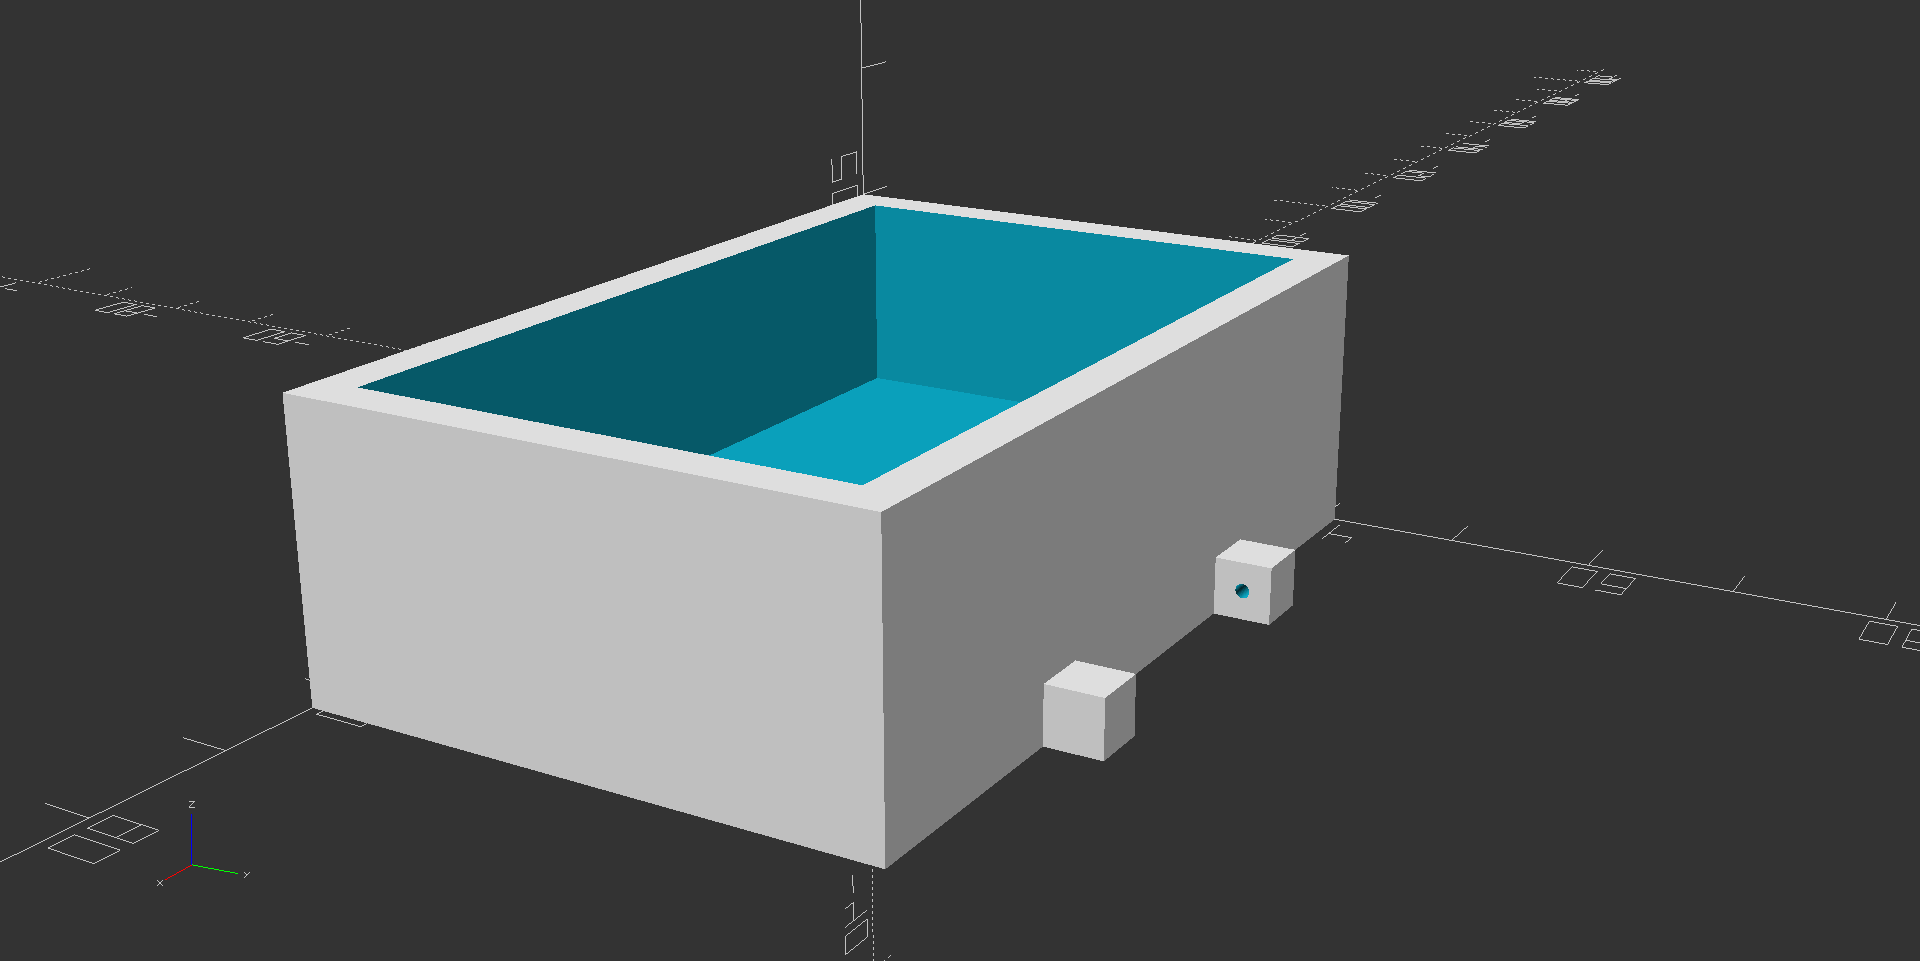
\includegraphics[width=\paperwidth]{images/enclosure.png}
}
\caption{Enclosure 3D Model}
\label{fig:enclosure}
\end{figure}